\chapter{Business research}
\label{chap:business-analysis}

\section{Industry growth}

2017 has been a year of exponential growth for the cryptographic asset market (term indicating the cryptocurrency market enabled by certain configurations of DLT). The outlook for 2018 seems to be set on the creation of solid regulatory frameworks required to provide consumer protection and guidelines.

Within less than a decade, the industry of cryptoassets has developed into a thriving ecosystem with a total market capitalization of over 300 billion USD.
The focus the cryptographic asset market is receiving through media and political coverage (Cryptoassets have topped the G20 agenda in March) has put increasing pressure on the actors playing in the market to match the needs and valuations from governance and financial institutions (the latter being players themselves).\\

It can be identified a drive from the investment banking industry (hereon sell-side) born out by the investment and participation in big consortia like R3 (which developed Corda) and DL platforms like Digital Asset. Institutional investors (hereon, buy-side) seem to be falling behind, and the risks this poses are of being presented with technology architectures with terms dictated by the sell-side self-interest.

The Bank of England identified this threat in a recent paper \textit{“…if a DL (or other) technological solution for settlement ultimately succeeds in replacing existing settlement methods,
it is likely to be characterized by network externalities and decreasing average costs. This suggests that the industry may well retain its high degree of concentration. It is possible and likely that a small number of Central Securities Depositories (CSDs) will be replaced by a small number of DL network providers and as a result future settlement services may be associated with some form of monopoly pricing”} \cite{bankofenglandreport}. The buy-side failure to action may end up delegating to the sell-side the most of the definition and development of DLT infrastructure, the sell-side being a party with potentially diverging interests from them, while if it actually ended up participating in the development and research of DLT it could add another strong player in the industry with a sizable budget to invest in the technology.

\begin{figure}[b]
    \begin{tcolorbox}[colframe=boxcolor]
        \section*{Sell-side and Buy-side}
        Sell-side and buy-side are terms belonging to the financial investment world.

        Sell-side refers primarily to the investment banking industry. It refers to the key function of the investment bank - namely helping companies to raise debt and equity capital and then sell those securities to investors. The investment bank role is that of a seller of corporate securities to institutional investors.

        Buy-side broadly refers to such institutional investors, such as mutual funds, hedge funds, insurance companies, endowments and pension funds. They raise money from investors and invest that money across various asset classes using a variety of different trading strategy.

        As of 2014 the estimated flow of money between the two sides is of approximately 227 trillion USD in global assets.
    \end{tcolorbox}
\end{figure}

\begin{figure}[t]
    \centering
    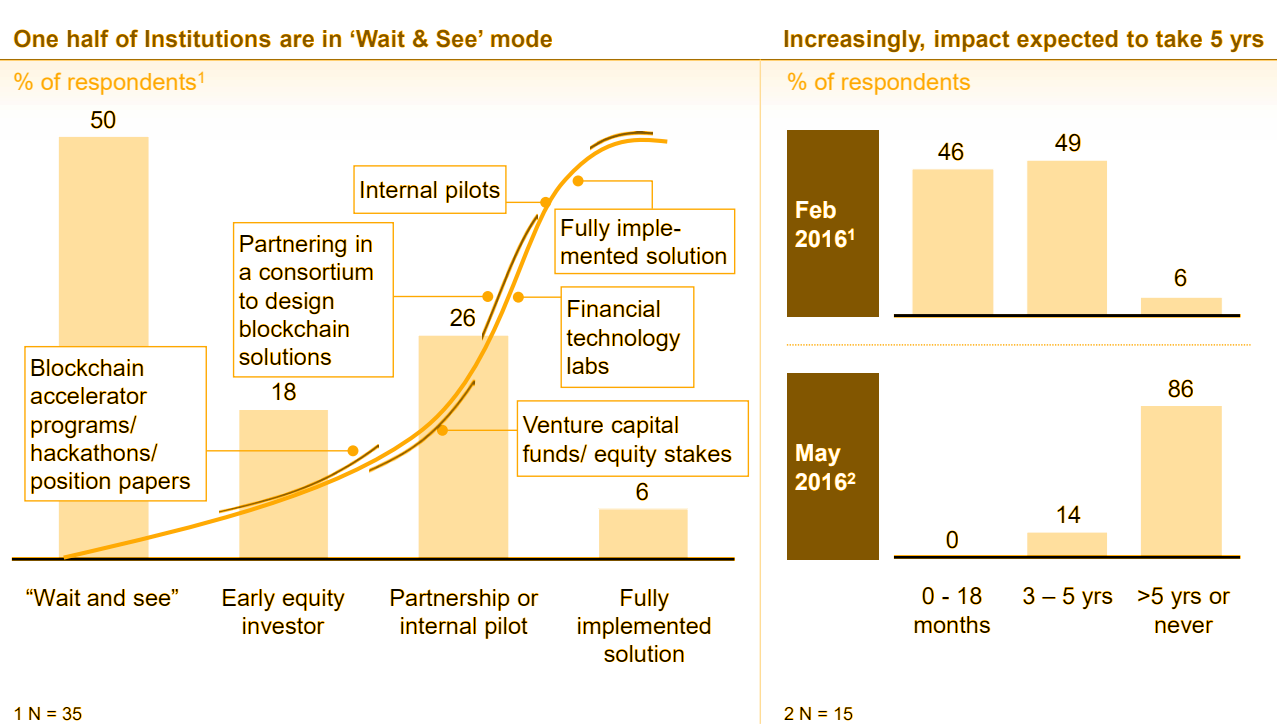
\includegraphics[scale=0.45]{dlt-industry-response}
    \caption{
        Infographic on the industry response to DLT, based on survey of senior executive leadership in financial institutions, Feb 2016 and May 2016, McKinsey \& Company.
        }
\end{figure}

\section{Governments stance}


It is fair to say that DLT has been on a steady rise in the governments' agenda in light of its saving, automatization and security advantages.
Central banks around the world are exploring DLT-based digital currencies - UK, Russia, Sweden, Canada and China's central banks are assessing risks and benefits of issuing fiat currencies backed by digital currencies, and investigating their potential effects on the economy and on financial stability.

The UK Government's Office of Science published a major report on DLT in January 2016, \cite{ukgovdltpaper}, assessing the possibilities of DLT use in private and public areas. The Department for Work and Pensions in the UK has been testing from June 2016 the use of DLT for welfare benefit payments, that trough a phone application lets welfare claimants manage their benefit money, having transaction recorded on a DL with the aim to create a more solid and efficient welfare infrastructure preventing frauds.

The Estonian government has been experimenting with DLTs for a long time, as apparent from its \cite{eresidency} platform, where it's possible to verify government records like birth or marriage certificates, which are only a couple of the services provided by, as the e-Residency project seem to be trying to encompass a whole variety of utilities, like opening a bank account or starting a company (in Estonia), but most importantly, providing a form of transnational digital identity, so far as to having NASDAQ partnering with the platform to enable secure e-voting in shareholders meetings.

By 2020 Dubai wants to become the first government in the world to conduct all of its transactions using blockchain. The emirate estimates that adding visa payments, license renewals and other documents to the blockchain could save 1.2 billion EUR annually in document processing alone, and also cut CO2 emissions and redistribute 25.1 million hours of economic productivity.

The European Union Intellectual Property Office (EUIPO) is investigating how blockchain could combat counterfeiting, which costs the EU about 60 billion EUR each year according to the agency. In June 2018 the EUIPO organized a Hackathon competition in Brussels to develop a series of anti-counterfeiting blockchain solutions, drawing support from specialists in law, IP and anti-counterfeiting. \\

Briefly, other relevant government-backed applications and researches include the USA's Food and Drug Administration's exploring blockchain solutions for patent sharing, Denmark's Liberal Alliance blockchain voting platform and Georgia's blockchain land registry project. 


\section{Financial stance}

The two biggest trends in DLT development seem to be:
\begin{enumerate}
    \item Commercial FinTech startups developing applications for different purposes utilizing public blockchain infrastructure, like BitCoin and Ethereum.
    \item Industry consortiums researching and developing private, permissioned distributed ledgers to address a set of industry-specific enterprise use-cases.
\end{enumerate}

A survey by Greenwitch Associates, \cite{greenwitchdltreport}, gathering 400 market participants (as in financial companies, funds, etc) working on DLT has tried to assess opinions on the key trends and issues in the current state of DLT development. The report finds engagement across the sample at 63\%, with Market Infrastructure providers in the high end with 75\% engagement, and Asset Managers in the bottom, with 32\% engagement.

This presents a picture of lagging in the adoption of the technologies, due to the competition of other competing technologies. According to a recent survey from \cite{multifundssurvey}, big data analytics, AI and robo-advice are currently higher up in the Asset Managers' agenda than DLT, accounting for more than half (55\%) of responses, explaining that it is "probably down to the fact that these new technologies are relatively easier to implement than more revolutionary DLT concepts". 

But as \cite{ibmdltreport} reports, recent evidence shows that the industry is notwithstanding operating in the research and development department. 
Examples (extrapolated from the report), include:

\begin{itemize}
    \item Schroders announcement that they have joined the Hyperledger Project
    \item Northern Trust’s implementation of a blockchain platform for Private Equity fund administration in partnership with Unigestion and IBM
    \item BlackRock’s announcement of their intention to Blockchain-enable Provider Aladdin, a private platform / dashboard to streamline transactions with BlackRock’s Custodians
    \item The launch of a Blockchain-based solution for syndicated loan servicing by Synaps (a joint venture of Ipreo and Symbiont), with involvement from Asset Managers including Eaton Vance and Alliance Bernstein
    \item Calastone’s launch of Blockchain-based distributed market infrastructure
    \item FNZ ‘s development of FNZChain as a private blockchain for Asset Management registers
    \item SETL’s launch of Iznes, in collaboration with various asset managers, as a Pan-European Distribution and Transfer Agent Platform for fund subscriptions, distributions and
    settlements
    \item The announcement from Natixis in July 2017 that they had successfully sold funds directly to clients through FundsDLT, a fund distribution platform developed by a partnership of the Luxembourg Stock Exchange / Fundsquare, InTech and KPMG;
    \item The news that SEB are working with NASDAQ on the development of a trading platform for Swedish mutual funds
    \item The rise of crypto fund launches in 2017, representing the fastest growth of any hedge fund sector in the industry’s history, \cite{hedgefundcryptoreport}
\end{itemize}
\clearpage

\section{Adoption considerations}

It is clear that many market players and public authorities have embarked on a learning process that has familiarized many of them with the foundations of DLT. Investment in the technology has started to gain momentum, and is expected to grow at a very high pace in the near future.

The technology has the potential to support attractive models for the tech-savvy generation of consumers who wants more control over their investments and finances, delivered via their favored media, thus providing a strong and agreeable user base.

The effective use case execution of said solution will depend highly on the collaboration among players in an ecosystem. In the financial services case, a strong interest has been outlined by banks and financial institutions and FinTech companies, with a 400 million USD estimated capital market spending by 2019. 
It is believed that right now the biggest challenge for DLT is going to be shaping a regulatory environment and the agreement on key standards and active collaboration across all required players.

It is hence believed that entering the market in this moment seems to be the prime time to ripe the benefits provided by the assessing ecosystem to solidify a strong and longstanding position among current and future competing solutions. Entering the market at this point in time - when the industry hasn't yet transformed itself - offers real potential that isn't ignorable, as most of the highest commercial gains expected for DLT will take place in the first transitional period after its stabilization in the market.

\begin{figure}[h]
    \centering
    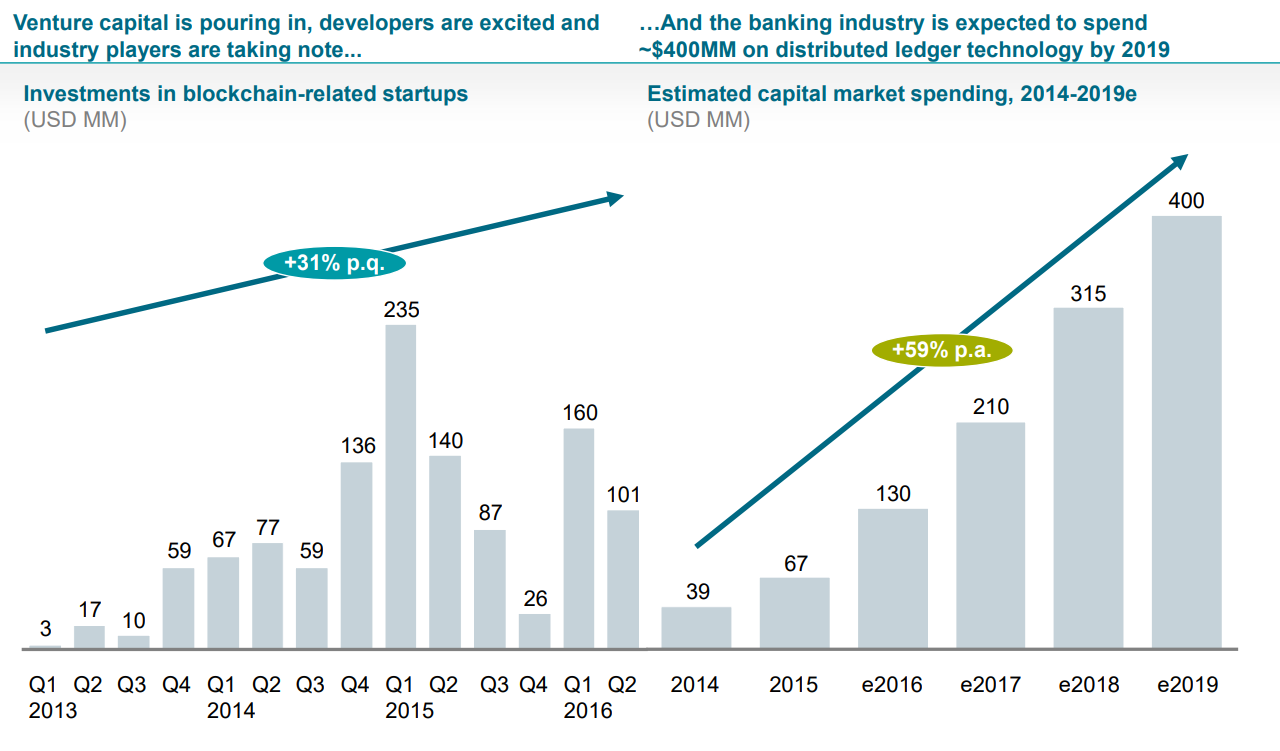
\includegraphics[scale=0.5]{dlt-investments}
    \caption{
        Infographic on the investments in DLT development,  based on data from AITE Group, Tabb Group, CoinDesk}
\end{figure}